\documentclass[11pt]{beamer}
\usetheme{Antibes}
\usepackage{ragged2e}
\title{FTech Training}
\subtitle{Using Beamer}
\author{Luc Nguyen}
\institute{HUST}
\date{\today}
\usetheme{Boadilla}

\begin{document}
\begin{frame}
	\frametitle{\textbf{LINEAR REGRESSION}}
	\framesubtitle{Idea}
			\pause
	\begin{itemize}
		\item Linear regression is a linear approach to modeling the relationship between a scalar response and one or more explanatory variables.
			\pause 
		\item Type of linear regression : 
		\begin{itemize}
			\item Simple linear regression : $ \hat{y} = xw + b $
			 \\ where $\hat{y}, x, w, b$ is a scalar variable.
			\item Multivariate linear regression : $ \hat{y} = xw + b = \bar{x}w$
			 \\ where $w, x$ are vectors, $\hat{y}, b$ is a scalar number.
		\end{itemize}
	\end{itemize}
\end{frame}
\begin{frame}
	\frametitle{\textbf{LINEAR REGRESSION}}
	\framesubtitle{Pros and Cons}
	\begin{minipage}[c]{0.5\textwidth}
	\begin{itemize}
		\item Pros
		\begin{itemize}
			\pause
			\item Quick
			\pause
			\item Easy to implement	
			\pause
		\end{itemize}
		\item Cons 
			\pause
		\begin{itemize}
			\item Essential to extract data to \textbf{independent} features
			\pause
			\item May drop relations between explanatories
			\pause
			\item Hard to scale with complicated, unlinear data
		\end{itemize}
	\end{itemize}
	\end{minipage}
	\begin{minipage}[c]{0.4\textwidth}
	\begin{center}
		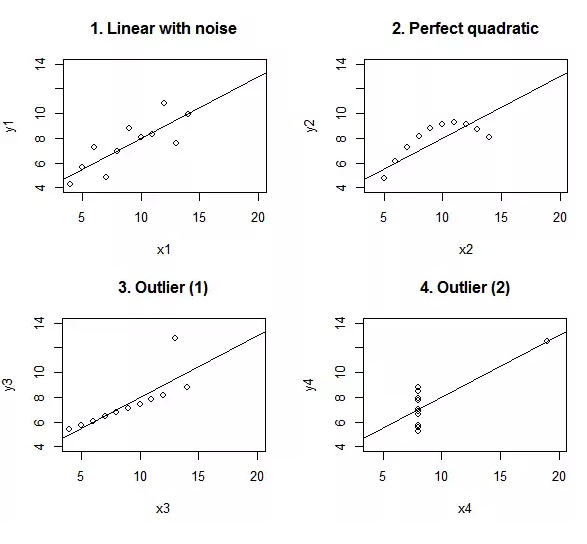
\includegraphics[width=\textwidth]{unLR.png}	
	\end{center}
		\end{minipage}

\end{frame}

\begin{frame}
	\frametitle{\textbf{LINEAR REGRESSION}}
	\framesubtitle{Model of Linear regression}
	 \begin{minipage}[c]{0.5\textwidth}
		  Mathematics model : 
			\pause
	\begin{itemize}
		\item Training data set : $Y$ and $X$
			\pause
		\item Need to find a matrix $W$ where $\hat{y} = Wx $ such that $\hat{y}$ most fit to $y$ in $Y$
	\end{itemize} 
	\end{minipage}		  
	\begin{minipage}{0.48\textwidth}		
		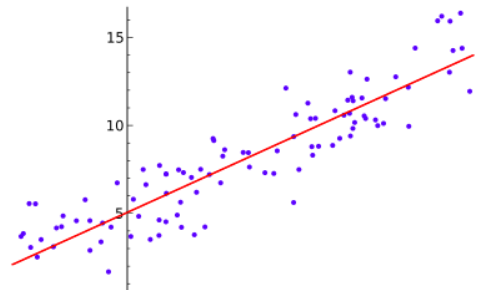
\includegraphics[width=\textwidth]{LR1.png} 
	\end{minipage}
	
\end{frame}
\begin{frame}
	\frametitle{\textbf{LINEAR REGRESSION}}
	\framesubtitle{Model of Linear regression}
	\begin{itemize}
		\item Lost function : 
		$$ \mathbb{L} = \dfrac{1}{2}\sum_{i=1}^N(y_i-\hat{y})^2 = \dfrac{1}{2}\sum_{i=1}^N(y_i-\hat{x}_iw)^2 = \dfrac{1}{2}\left\|y-\bar{X}w\right\|^2_2 $$
			\pause
		\item Derivative : 
		$$  \dfrac{\partial\mathbb{L}(w)}{\partial w} = \bar{X}^T \left( \bar{X}w-y \right) $$
			\pause
		\item Minimum at :  $$ w = \left(\bar{X}^T\bar{X}\right)^{-1}\bar{X}^Ty $$
	\end{itemize}

\end{frame}
\end{document}